\chapter{ Выполнение работы}
\label{cha:analysis}

\section{ Четвертое задание}
Напишите результат вычисления выражений. Выполнение задания представлено в \ref{lst:4task}
\begin{lstlisting}[style=lispStyle, caption={Выражения и их результат},
                label={lst:4task}]
(list 'Fred 'and Wilma)
;Ошибка

(list 'Fred'(and Wilma))
;(A (B C))

(cons Nil Nil)
(Nil)

(cons T Nil)
(T)

(cons Nil T)
(Nil . T)

(list Nil)
(Nil)

(cons (T)Nil)
;Ошибка, T - воспринимается как функция

(list '(one two)'(free temp))
;((one two) (free temp))


(cons 'Fred'(and Wilma))
;(Fred and Wilma)

(cons 'Fred'(Wilma))
;(Fred Wilma)

(list Nil Nil)
;(Nil Nil)

(list T Nil)
;(T Nil)

(cons T(list Nil))
;(T Nil)

(list (T)Nil)
;Ошибка, функция T неопределена

(cons `(one two)'(free temp))
;((one two) free temp)
\end{lstlisting}

\section{ Пятое задание}
\textbf{Написать функцию (f ar1 ar2 ar3 ar4), возвращающую список \ref{eq:func}}
\begin{align}
((ar1\ ar2)(ar3\ ar4)) \label{eq:func}
\end{align}
%\begin{equation}
%\label{eq:func}
%\end{equation}

Листинг функции представлен в \ref{lst:1task}, результат в виде списочных ячеек представлен на схеме \ref{fig:4args}

\begin{lstlisting}[style=lispStyle, caption={Представление реализации функции (f ar1 ar2 ar3 ar4).},
                    label={lst:1task}]
(defun f (a b c d)
    (cons (list a b) (list (list c d))))
\end{lstlisting}

\begin{figure}[ht!]
    \centering{
        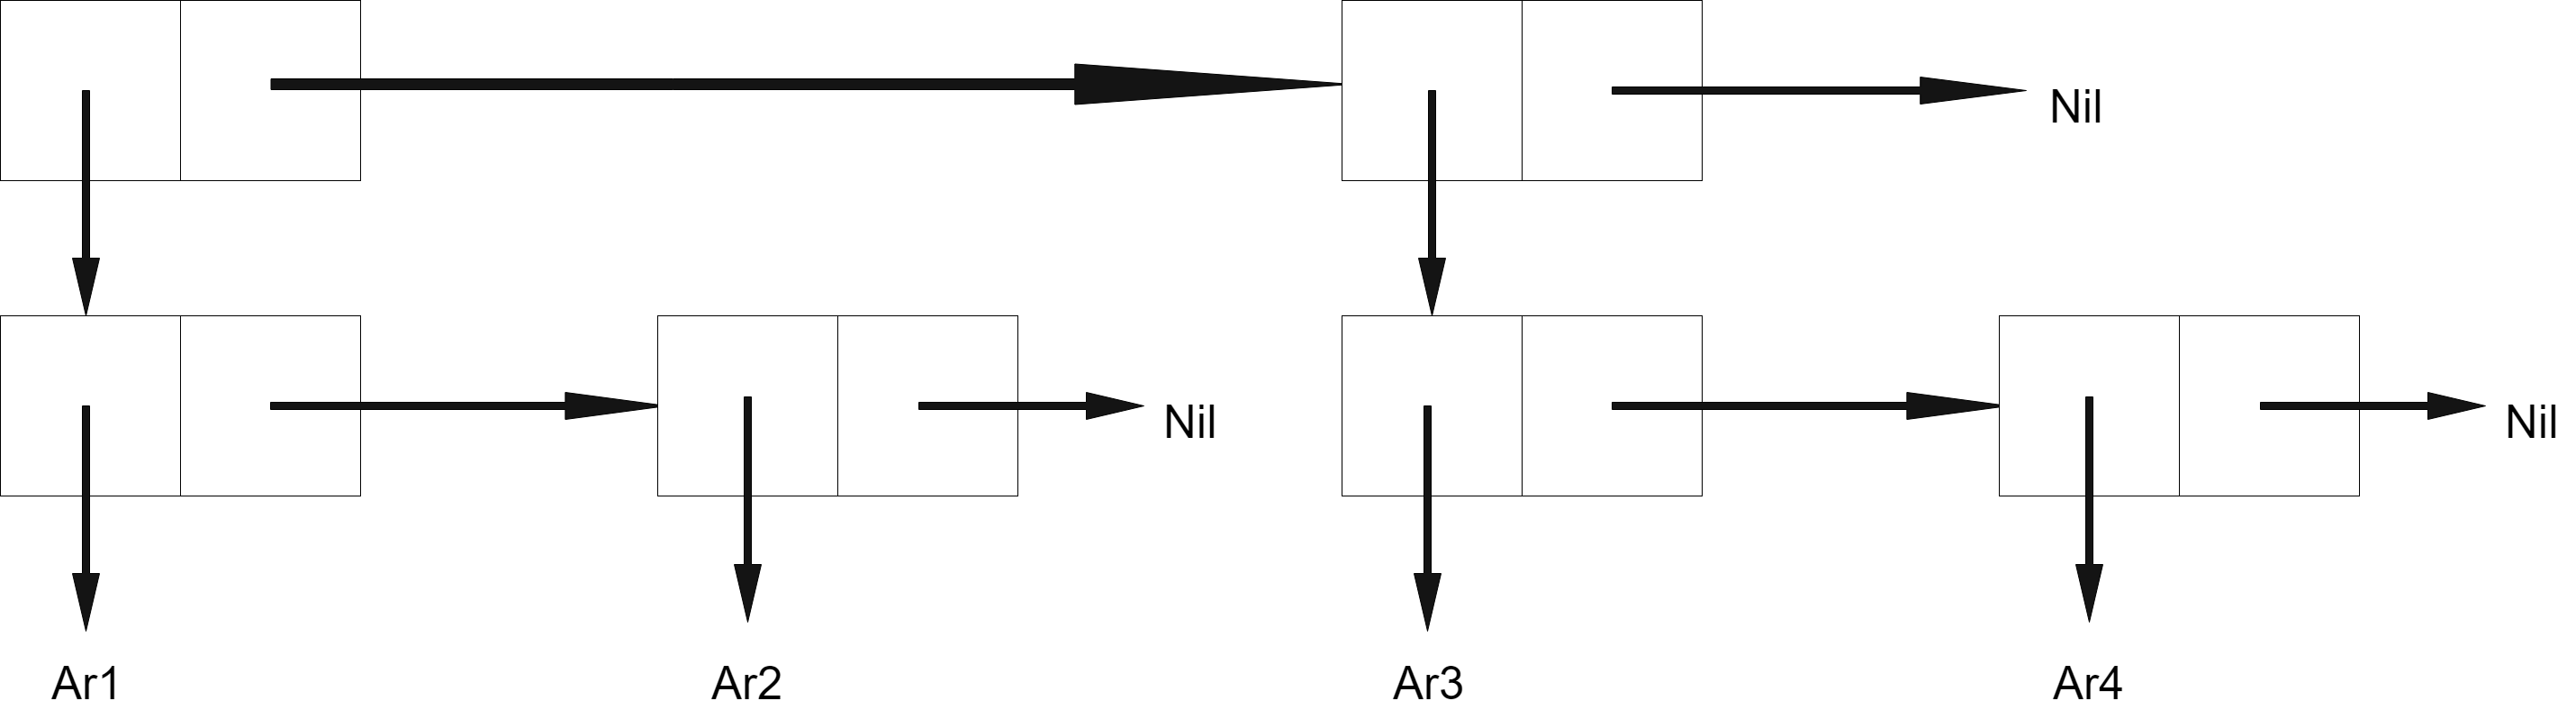
\includegraphics[width=1\textwidth]{img/4args.png}
        \caption{ Представление результата функции (f ar1 ar2 ar3 ar4) в виде списочных ячеек}
        \label{fig:4args}
    }
\end{figure}

\textbf{Написать функцию (f ar1 ar2), возвращающую список \ref{eq:func2}}
\begin{equation}
\label{eq:func2}
((ar1)(ar3))
\end{equation}

Листинг функции представлен в \ref{lst:2task}, результат в виде списочных ячеек представлен на схеме \ref{fig:2args}

\begin{lstlisting}[style=lispStyle, caption={Представление реализации функции (f ar1 ar2).},
                    label={lst:2task}]
(defun f (a b)
    (cons (list a) (list (list b))))

\end{lstlisting}

\begin{figure}[ht!]
    \centering{
        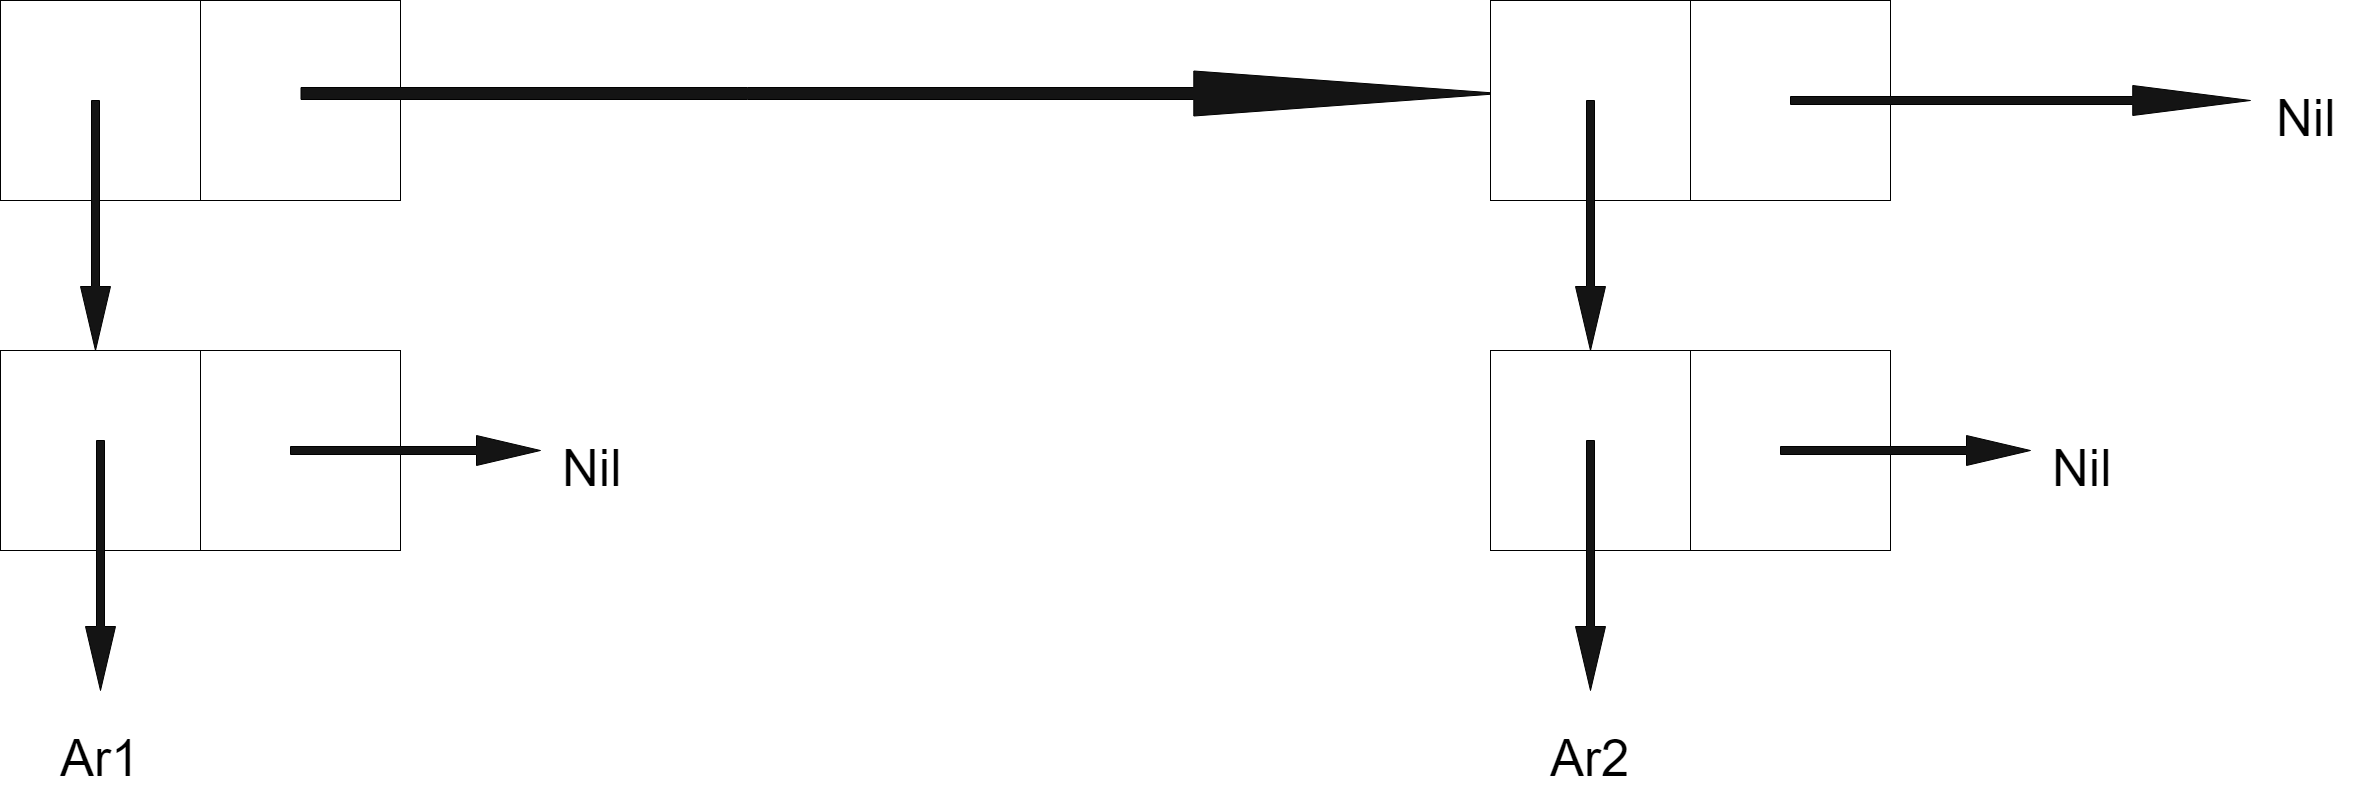
\includegraphics[width=1\textwidth]{img/2args.png}
        \caption{ Представление результата функции (f ar1 ar2) в виде списочных ячеек}
        \label{fig:2args}
    }
\end{figure}


\textbf{Написать функцию (f ar1), возвращающую список \ref{eq:func3}}

\begin{equation}
\label{eq:func3}
(((ar1)))
\end{equation}

Листинг функции представлен в \ref{lst:3task}, результат в виде списочных ячеек представлен на схеме \ref{fig:1arg}

\begin{lstlisting}[style=lispStyle, caption={Представление реализации функции (f ar1).},
                    label={lst:3task}]
(defun f (a)
    (list (list (list a))))

\end{lstlisting}

\begin{figure}[ht!]
    \centering{
        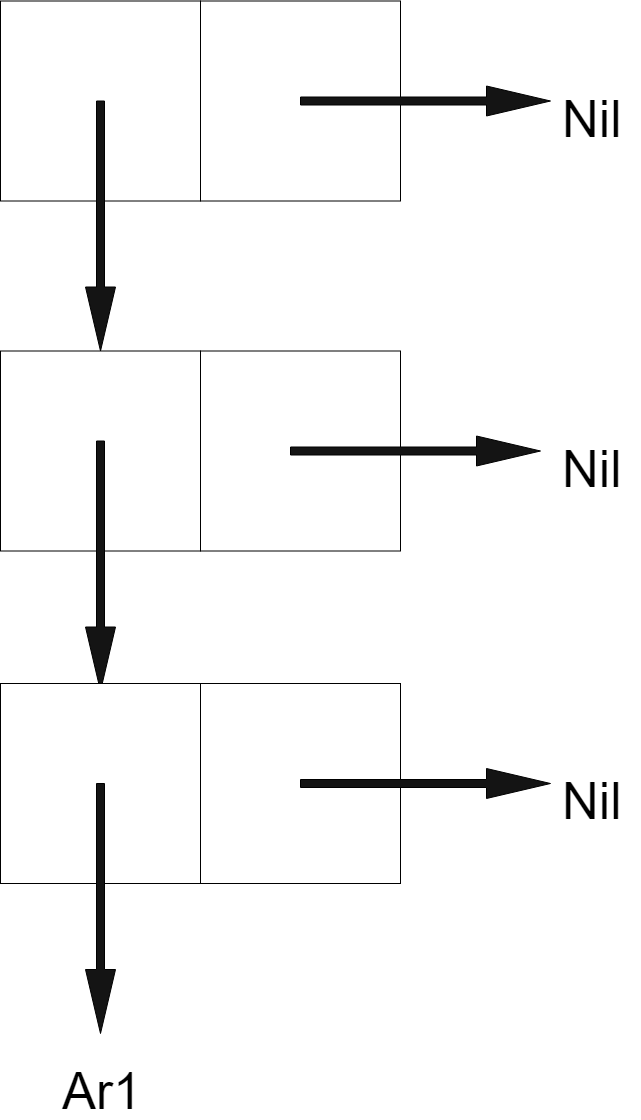
\includegraphics[width=.4\textwidth]{img/1arg.png}
        \caption{ Представление результата функции (f ar1) в виде списочных ячеек}
        \label{fig:1arg}
    }
\end{figure}


